%% IFBThesis Latex Template Version 1.0, a fork of :
%% 	RiSE Latex Template - version 0.5
%%
%% IFBthesis latex template for thesis and dissertations
%% https://github.com/auyer/IFBtcc
%%
%% (c) 2017 Rafael de Campos Passos (rcpassos@ieee.org)
%%
%% This document was initially based on RiSE Latex template, from Yguaratã
%% Cerqueira Cavalcanti
%%
%% GENERAL INSTRUCTIONS
%%
%% We strongly recommend you to compile your documents using pdflatex command.
%% It is also recommend use the texlipse plugin for Eclipse to edit your documents.
%%
%% Options for \documentclass command:
%%         * Idiom
%%           pt   - Portguese (default)
%%           en   - English
%%
%%         * Text type
%%           bsc  - B.Sc. Thesis
%%           msc  - M.Sc. Thesis (default)
%%           qual - PHD qualification (not tested yet)
%%           prop - PHD proposal (not tested yet)
%%           phd  - PHD thesis
%%
%%         * Media
%%           scr  - to eletronic version (PDF) / see the users guide
%%
%%         * Pagination
%%           oneside - unique face press
%%           twoside - two faces press
%%
%%		   * Line spacing
%%           singlespacing  - the same as using \linespread{1}
%%           onehalfspacing - the same as using \linespread{1.3}
%%           doublespacing  - the same as using \linespread{1.6}
%%
%% Reference commands. Use the following commands to make references in your
%% text:
%%          \figref  -- for Figure reference
%%          \tabref  -- for Table reference
%%          \eqnref  -- for equation reference
%%          \chapref -- for chapter reference
%%          \secref  -- for section reference
%%          \appref  -- for appendix reference
%%          \axiref  -- for axiom reference
%%          \conjref -- for conjecture reference
%%          \defref  -- for definition reference
%%          \lemref  -- for lemma reference
%%          \theoref -- for theorem reference
%%          \corref  -- for corollary reference
%%          \propref -- for proprosition reference
%%          \pgref   -- for page reference
%%
%%          Example: See \chapref{chap:introduction}. It will produce
%%                   'See Chapter 1', in case of English language.
%%
%% Citation commands:
%%          \citet (from natbib) -- To cite a reference as part of the narrative
%%          \citep (from natbib) -- To cite a reference between parenthesis
%%          citationblock environment -- To produce direct citation blocks according to the ABNT

\documentclass[pt,twoside,onehalfspacing,bsc]{ifgtcc}


\usepackage{colortbl}
\usepackage{color}
\usepackage[table]{xcolor}
\usepackage{microtype}
\usepackage{bibentry}
\usepackage{subfigure}
\usepackage{multirow}
\usepackage{rotating}
\usepackage{booktabs}
\usepackage{pdfpages}
\usepackage{caption}
\usepackage{lipsum}
\usepackage{sectsty}
%pages
\usepackage{lastpage}
\usepackage{float}

%% Set the language used in your code in the block above

\captionsetup[table]{position=top,justification=centering,width=.85\textwidth,labelfont=bf,font=footnotesize}
\captionsetup[lstlisting]{position=top,justification=centering,width=.85\textwidth,labelfont=bf,font=footnotesize}
\captionsetup[figure]{position=bottom,justification=centering,width=.85\textwidth,labelfont=bf,font=footnotesize}

%% Chapter and (Sub)Section fonts must be same size as text (12)
\sectionfont{\fontsize{12}{15}\selectfont}
\subsectionfont{\fontsize{12}{15}\selectfont}
\subsubsectionfont{\fontsize{12}{15}\selectfont}

%% Change the following pdf author attribute name to your name.
\usepackage[linkcolor=black,
            citecolor=black,
            urlcolor=black,
            colorlinks,
            pdfpagelabels,
            pdftitle={Rise Thesis Template (ABNT)},
            pdfauthor={Rise Thesis Template (ABNT)},
            breaklinks=true]{hyperref}

\address{FORMOSA}

\universitypt{Instituto Federal de Goiás}
\universityen{Federal Institute of Goi\'as}

\campus{{\it Campus} Formosa}

\departmentpt{Departamento de Áreas Acadêmicas}
\departmenten{Academic Department}

\programpt{Análise e Desenvolvimento de Sistemas}
\programen{Systems Analyses and Develpment}

\majorfieldpt{Ciência da Computação}
\majorfielden{Computer Science}

\title{Meu TCC}

\date{2019}

\author{Aluno da Silva}
\adviser{Prof. Dr. Waldeyr Mendes Cordeiro da Silva}
%\coadviser{Nome dompleto do co-orientador }

% Macros (defines your own macros here, if needed)
\def\x{\checkmark}
%\let\lstlistoflistings\origlstoflistings
\begin{document}

\frontmatter

\frontpage

\presentationpage

\begin{fichacatalografica}
\FakeFichaCatalografica % Comment this line when you have the correct file
%\includepdf{fig_ficha_catalografica.pdf} % Uncomment this
\end{fichacatalografica}


%NAO APAGAR ISSO AQUI
%\banca

\begin{ata}
\begin{figure}
	\centering 
	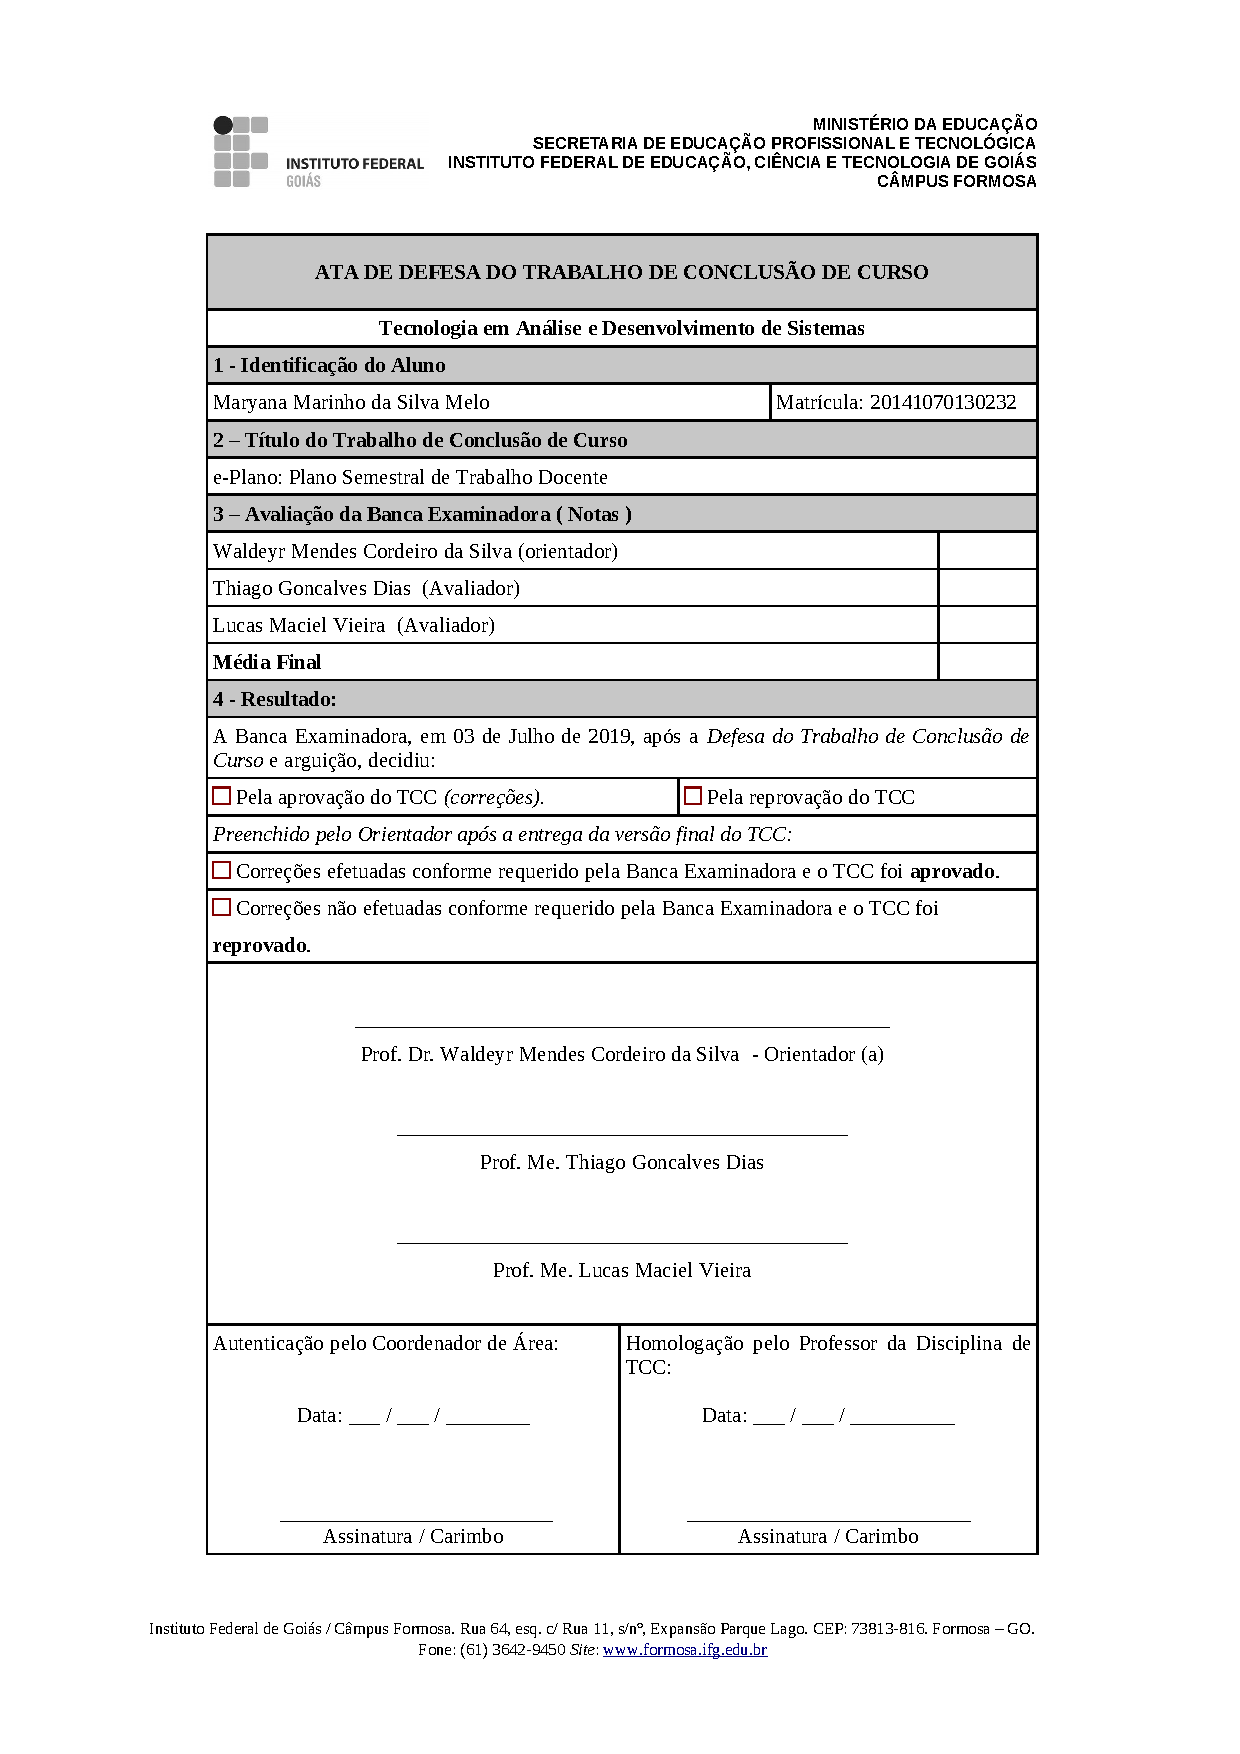
\includepdf[pages=-,width=\textwidth]{doc/ModeloAta.pdf}
\end{figure}
\end{ata}


\begin{ata}
	\begin{figure}
		\centering 
		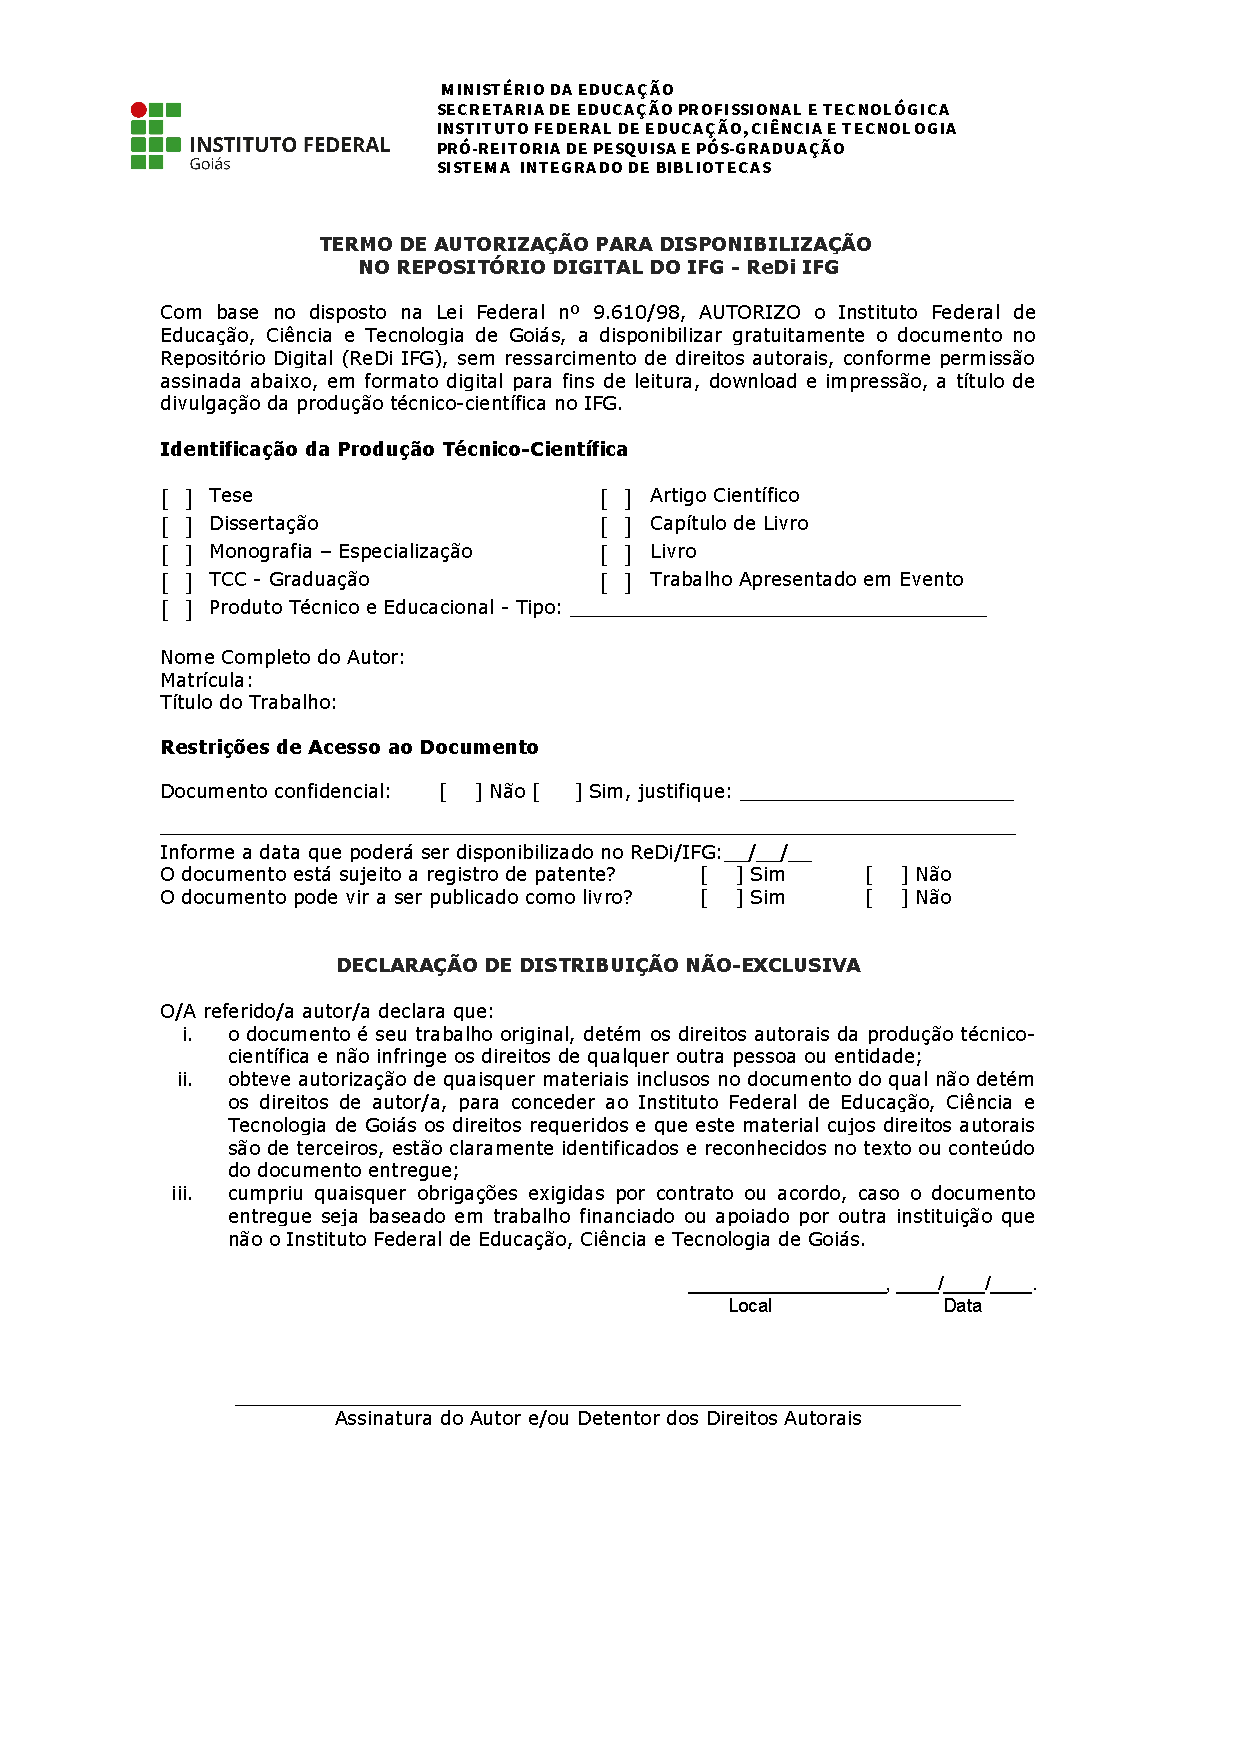
\includepdf[pages=-,width=\textwidth]{doc/redi.pdf}
	\end{figure}
\end{ata}


\begin{dedicatory}
Eu dedico ...
\end{dedicatory}

% \acknowledgements
% \lipsum[1-4]

Agradeço a minha mãe por me apoiar sempre, e por fazer eu chegar ate aqui. Sem ela não seria possível.
Ao meu orientador professor Dr. Waldeyr Mendes Cordeiro da Silva, pelo conhecimento, orientação e compreensão.
Aos meus amigos pelo apoio, incentivo e torcida pelo meu sucesso.
A todos que me ajudaram direta ou indiretamente nessa nessa jornada. 


% \begin{epigraph}[]{Márcio de Deus}
% When one finds a hard problem, the more complicated it is, the more one ought to work towards enlightening it's solution.
% \end{epigraph}

\resumo
% Escreva seu resumo no arquivo resumo.tex
{\parindent0pt
	O resumo é um texto que deve sumarizar o trabalho.
Use frases curtas e autocontidas. 
Encadeie-as mostrando o contexto do seu trabalho, o problema, a hipótese ou solução proposta, os pontos importantes do método e dos resultados.
O resumo deve ser escrito em um parágrafo único, portanto, é recomendado escrevê-lo após o texto estar pronto. 
O resumo é seguido de palavras chaves definidas no arqivo tcc.tex.

\begin{keywords}
TCC, IFG, modelo 
\end{keywords}
}

\abstract
% Write your abstract in a file called abstract.tex
{\parindent0pt
	O abstract é o resumo em língua Inglesa. 
Embora o conteúdo apresentado seja o mesmo, não deve ser a tradução literal.

\begin{keywords}
TCC, IFG, model
\end{keywords}
}

% List of figures
\listoffigures

% List of Codes
%\lstlistoflistings

% List of tables
\listoftables

% List of acronyms
% Acronyms manual: http://linorg.usp.br/CTAN/macros/latex/contrib/acronym/acronym.pdf
\listofacronyms
\begin{acronym}[ACRONYM] 
% Não é necessário ordenar as siglas
\acro{IFG}[IFG]{Instituto Federal de Educação, Ciência e Tecnologia de Goiás}
\acro{DAA}[DAA]{Departamento de Áreas Acadêmicas}
\acro{Cefet}[Cefet]{Centros Federais de Educação Profissional e Tecnológica}
\acro{Uneds}[Uneds]{Unidade de Ensino Descentralizada}
\acro{ETFG}[ETFG]{Escola Técnica Federal de Goiás}
\acro{URL}[URL]{Uniform Resource Locator}
\acro{HTML}[HTML]{Hypertext Markup Language}
\acro{CSS}[CSS]{Cascading Style Sheets}
\acro{SGBDs}[SGBDs]{Sistema de Gerenciamento de Banco de Dados}
\acro{SQL}[SQL]{Structured Query Language}
\acro{NoSQL}[NoSQL]{Not Only SQL}
\acro{REST}[REST]{Representational State Transfer}
\acro{HTTP}[HTTP]{Hypertext Transfer Protocol}
\acro{URI}[URI]{Uniform Resource Identifier}
\acro{JSON}[JSON]{JavaScript Object Notation}
\acro{PDF}[PDF]{Portable Document Format}
%%
\acro{afm}[AFM]{Alphabet Frequency Matrix}
\acro{api}[API]{Application Programming Interface}
\acro{arima}[ARIMA]{Auto-Regressive Integrated Moving Average}
\acro{brn}[BRN]{Bug Report Network}
\acro{bts}[BTS]{Bug Triage System}
\acro{cas}[CAS]{Context-Aware Systems}
\acro{ccb}[CCB]{Change Control Board}
\acro{cr}[CR]{Change Request}
\acro{cvs}[CVS]{Concurrent Version System}
\acro{es}[ES]{Expert System}
\acro{floss}[FLOSS]{Free/Libre Open Source Software}
\acro{glr}[GLR]{Generalized Linear Regression}
\acro{gqm}[GQM]{Goal Question Metric}
\acro{html}[HTML]{HyperText Markup Language}
\acro{ir}[IR]{Information Retrieval}
\acro{irt}[IRT]{Recôncavo Institute of Technology}
\acro{jdt}[JDT]{Jazz Duplicate Finder}
\acro{lda}[LDA]{Latent Dirichlet Allocation}
\acro{loc}[LOC]{Lines of Code}
\acro{lsi}[LSI]{Latent Semantic Indexing}
\acro{ms}[MS]{Mapping Study}
\acro{msr}[MSR]{Mining Software Repositories}
\acro{nlp}[NLP]{Natural Language Processing}
\acro{promise}[PROMISE]{Predictive Models in Software Engineering}
\acro{rbes}[RBES]{Rule-Based Expert System}
\acro{rhel}[RHEL]{RedHat Enterprise Linux}
\acro{saas}[SaaS]{Software as a Service}
\acro{scm}[SCM]{Software Configuration Management}
\acro{serpro}[SERPRO]{Brazilian Federal Organization for Data Processing}
\acro{slr}[SLR]{Stepwise Linear Regression}
\acro{slr}[SLR]{Systematic Literature Review}
\acro{svd}[SVD]{Singular Value Decomposition}
\acro{svm}[SVM]{Support Vector Machine}
\acro{svn}[SVN]{Subversion}
\acro{tfidf}[TF-IDF]{Term Frequency-Inverse Document Frequency}
\acro{vsm}[VSM]{Vector Space Model}
\acro{xp}[XP]{Extreming Programming}
\acro{gui}[GUI]{Graphical User Interface}
\end{acronym}

% Summary (tables of contents)
\tableofcontents

\mainmatter

\chapter{Introdução}\label{Introducao}

Este documento serve de exemplo da utilização da classe IFG para escrever um texto cujo objetivo é apresentar os resultados de um trabalho científico. 
Este modelo foi produzido a partir do modelo de monografia do \href{https://github.com/UnB-CIC/Monografia}{Departamento de Ciência da Computação da UnB}.

Na introdução, o autor deve apresentar os fatos e fatores que influenciam o contexto do trabalho.
Em seguida, o autor deve mostrar seu problema nesse contexto em um último parágrafo.
Os objetivos devem ser destacados em uma subseção.
Citações são mais do que uma obrigação, são o reconhecimento e respeito pelo trabalho dos nossos colegas de ciência.

Para citar assim:~\citep{Silva2018graph}, Escreva assim:

\begin{verbatim}
~\citep{Silva2018graph}
\end{verbatim}

Para citar assim:~\cite{Silva2018graph}, Escreva assim:

\begin{verbatim}
~\cite{Silva2018graph}
\end{verbatim}


\section*{Objetivo}

Objetivos normalmente iniciam-se com verbos no infinitivo, por exemplo: 

Escrever um bom TCC.

\subsection*{Objetivos Específicos}

\begin{enumerate}
	\item Fazer AAAA
	\item Implementar BBBB
	\item Produzir CCCC
\end{enumerate}

Alguns cuidados devem ser tomados para melhorar a experiência do leitor.
O primeiro deles é sempre usar referências cruzadas de siglas, capítulos e seções, figuras e tabelas.
O nome a seguir: \acf{IFG}, é um exemplo de uso de siglas para ser usado na primeira citação.
\ac{IFG} é apenas a sigla, após seu primeiro uso.
Este é um exeplo de nota de rodapé\footnote{\url{https://www.capes.gov.br/images/stories/download/diversos/OrientacoesCapes_CombateAoPlagio.pdf}}.

\section{Descrição Dos Capítulos}

A última parte da introdução é uma descrição do que o leitor encontrará em cada capítulo.
Por exemplo, no \nameref{Referencial_Teorico} são apresentados comandos em \LaTeX e dicas para formatar seu TCC.
No \nameref{Metodo} é descrito o método utilizado para alcançar os objetivos listados aqui.
O \nameref{Resultados} apresenta os resultados obtidos.
No \nameref{Conclusao}, são apresentadas as conclusões, contribuições científicas e trabalhos futuros.



\chapter{Referencial Teórico}
\label{Referencial_Teorico}


Este capítulo oferece sugestões para descrever o referencial teórico.

\section{O que devo escrever aqui?}%

Descreva aqui tudo que for pertinente a seu trabalho com o máximo de detalhes e citando as respectivas fontes.

Você pode organizar este capítulo em seções:

\begin{verbatim} \section \end{verbatim}

e subseções: 

\begin{verbatim} \subsection \end{verbatim}
\chapter{Método}
\label{Metodo}
\indent
Este capítulo oferece sugestões para descrever o método.

\section{O que devo escrever aqui?}%

Cada ferramenta, tecnologia, definições e todo o arcabouço teórico do trabalho deve estar em seu \nameref{Referencial_Teorico}.
Aqui, no \nameref{Metodo} você deve escrever como utilizou as ferramentas, tecnologias e outros recursos para resolver o problema proposto com vistas a alcançar seus objetivos.
Este não é lugar para definir nada novo.


Não caia na tentação de dizer aqui os resultados! Guarde-os para o \nameref{Resultados}. Muitas vezes é interessante começar a escrita, justamente pelo \nameref{Resultados}.

\fontshape{n}\selectfont%
A tabela com a listagem de todas as atividades, pontuação e somatório encontra se na página de finalização do formulário.


\chapter{Resultados}
\label{Resultados}

Este capítulo deve mostrar o que você conseguiu alcançar após aplicar seu método em busca do seu Objetivo.

\section{O que devo escrever aqui?}
Bem, quando você iniciou seu trabalho, você tinha um problema claro a resolver.
Você pesquisou a respeito do seu problema e também a respeito de ferramentas, tecnologias e outros recursos que poderiam ajudá-lo a resolver seu problema. No método você estabelecu os passos usados para resolver o problema. Agora é hora de mostrar em detalhes que você alcançou os objetivos definidos na \nameref{Introducao}.

Oriente-se pelos Objetivos. Descreva em detalhes o seu sucesso!!
\chapter{Conclusão}
\label{Conclusao}

Esta é a conclusão do trabalho. 
Aqui são mostradas as contribuições para a ciência ou para a área em que se aplica a solução desenvolvida.
Também é importante mostrar os limites da contribuição e como eles podem ser rompidos em trabalhos futuros.

% References

\begin{references}
  \bibliography{bib/references}
\end{references}

% Appendix
\theappendix



\end{document}
